\section{Discussion and Future Work}
\label{sec:discussion}

% Summarize, restate contributions.
In this paper, we present a probabilistic approach to automatically coloring 2D patterns. We develop a factor graph model that is trained on example pattern colorings to statistically capture their coloring style and sampled using MCMC to generate a variety of pattern coloring suggestions. We demonstrate the utility of the model on a range of coloring tasks, and a perceptual study showed that the colorings it generates compare favorably to artist-created colorings.

% Discuss limitations, etc.
The model as presented has some limitations. In particular, the current model does not capture any semantic constraints on pattern regions, such as skies being blue or plants being green. This is not always a problem, as even human artists do not always respect these semantics (see the red clouds in Figure~\ref{fig:permutation}b), and patterns often admit many attractive, non-semantic colorings (Figure~\ref{fig:constrainedInference}). However, some patterns appear ugly or confusing when their colorings do not respect semantics, as shown in Figure~\ref{fig:badFlowers}. Labeling regions with semantic tags could address this problem, as the system could search for images on the web using these tags and build up a distribution of expected colors. It might even be possible to predict such labels automatically using sketch classification techniques~\cite{SketchClassification}.~\remark{Also discuss limitations implied by the results of our Turk study?} 

\begin{figure}
\centering
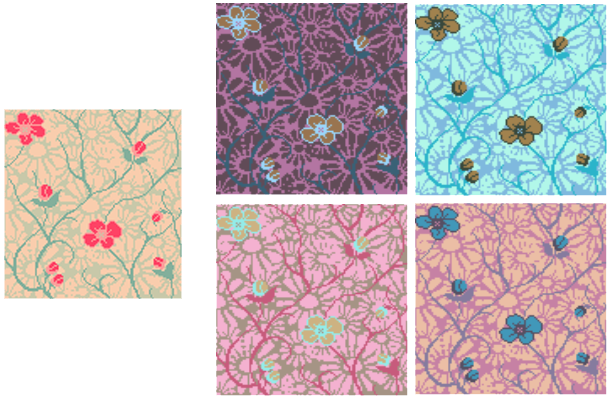
\includegraphics[width=0.7\columnwidth]{figs/badFlowers}
\caption{(Left) An artist's coloring of a pattern. (Right) High-scoring colorings of the same pattern sampled from our model. When the colorings do not respect the semantics of the flower stems by making them biologically impossible colors, it becomes difficult to parse the resulting image as one depicting a cluster of flowers.}
\label{fig:badFlowers}
\end{figure}

% Future work: Templatizing images
This research opens up several interesting avenues for future work.
First, the results demonstrated in this paper use patterns from Colourlovers or renderings that can be easily coerced into the same format. What if any image found `in the wild' could serve as a recolorable pattern template? As a simple first approach, we could extract a color theme from the image, and then quantize the image using the theme's colors~\cite{SharonPaletteExtraction}. Such a simple approach is unlikely to perform well on complex images that use many distinct colors, however. Solving the problem in general requires further research.

% Future work: Patterns where color groups are unknown
Second, this work explores colorizing patterns of the `color-by-numbers' format, in which some pattern regions are constrained to take the same color. What if this assumption were relaxed; that is, what if the color groups in the pattern template are unknown? A system that supported this more general type of pattern template could operate on an even larger set of inputs---essentially any image composed of segments. Implementing such a system would require a more sophisticated model, as well as transdimensional inference techniques to generate sample recolorings when the number of color groups is variable~\cite{ReversibleJumpMCMC}.

% Future work: Embed in real creative software
Finally, the prospect of embedding automatic coloring suggestion into real creative software presents an exciting opportunity. For example, a vector art program could continually generate suggestions in the background while its user works on a pattern; the user could choose to view the suggestions at any time, potentially picking one to use as an `autocompletion' of her work-in-progress. These kinds of tools have the potential to drastically shift the way that artists and enthusiasts work with color on a daily basis. 

%Discuss...stuff.
%Some suggestions:
%\begin{itemize}
%\item{How many training images are needed? (though maybe this should be part of the results section. We could look at the change in weight/coefficient differences as the number of training examples increases. Or possibly the fluctation in model score as number of training images increases?)}
%\item{What the model does well and what doesn't it do well? (i.e. maybe it does better on certain types of patterns?) }
%\end{itemize}
%
%
%Some ideas for future work:
%\begin{itemize}
% \item{Beyond a fixed number of color groups: Transdimensional inference.}
%  \item{Working with vector artwork, instead of bitmaps...They are much cleaner. Vector/layered artwork is also interesting due to possible blending effects (like mentioned below). Though one good thing about using bitmaps is that they are more readily available.}
% \item{More sophisticated templates and/or model: `Soft' segments with `soft' membership in color groups? Useful for color blending, dealing with more sophisticated artwork.}
% \item{Templatizing images: In line with the above..automatically or semi-automatically generating pattern templates from images. In our training set, we're provided the source color palette, but for other images, we don't necessarily have that. Currently, we could extract a color theme from the image using K-means or some other technique, and then do a quantization, but this is not very sophisticated and doesn't work well for complicated patterns}
% \item{Semantics: use the web to associate color distributions with labels, so that a user can label a region as 'skin' and we can respect that}
%\end{itemize}